\documentclass[a4paper]{article}
\usepackage{algorithmicx}
\usepackage{algpseudocode}
\usepackage{graphicx}
\usepackage{vmargin}
\usepackage[utf8]{inputenc}
\usepackage{mdwlist}
\setpapersize{A4}
\setmargins{2.5cm}       % margen izquierdo
{1.5cm}                        % margen superior
{16.5cm}                      % anchura del texto
{23.42cm}                    % altura del texto
{10pt}                           % altura de los encabezados
{1cm}                           % espacio entre el texto y los encabezados
{0pt}                             % altura del pie de página
{2cm}  


\begin{document}

\section{Plan de Vuelo}
\subsection{Problema a resolver}

Se cuenta con una cantidad n, entero no negativo, de vuelos disponibles. Cada vuelo se realiza de una ciudad a otra, y para cada uno se conoce la hora de salida y la hora de llegada respectivamente.
 El objetivo del problema es que dadas dos ciudades por ejemplo: X (origen) e  Y (destino).  Se devuelva un itinerario con los vuelos necesarios para llegar desde origen a destino, siempre que sea posible.  De esta manera el primer vuelo que realice el itinerario devuelto debe ser desde X, y el último debe tener como lugar de llegada a Y. Para efectuar este recorrido es posible tomar cualquier cantidad de vuelos intermedios cuya combinación me permita llegar a destino. Pero, siempre que entre los vuelos elegidos, el horario de  llegada a una ciudad y el horario del próximo vuelo que se efectué  desde la misma, haya como mínimo dos horas de diferencia (el horario de salida y de llegada es la cantidad de horas que faltan para realizar cada una de las acciones desde el momento en que se realiza la consulta). 
Se considerada solución óptima del problema a aquel itinerario que cumpla con lo descripto. Pero además, en el itinerario devuelto la llegada a destino se realice lo antes posible dee entre todos los itinerarios posibles que lleguen a Y partiendo desde X como primer vuelo.\newline

Ejemplo 1:

X Y 1\newline
vuelos:
1) X Y 10 12\newline
\vspace{1cm}
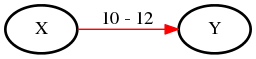
\includegraphics[width=\textwidth,height=0.5in,keepaspectratio
]{ejemplo1.png}\newline
\textit{Ejemplo representado como digrafo donde cada nodo representa a una ciudad. La arista hacia donde parte el vuelo, desde la ciudad en la que me encuentro. Ademas en la misma se detalla la hora de salida y llegada. Con rojo se indican los vuelos que debo tomar para resolver el problema.} \newline

En este ejemplo se desea llegar de X a Y y se provee de un vuelo. El mismo se realiza desde la ciudad X partiendo a 10 horas de realizada la consulta y se llega a la ciudad Y dos horas después de la partida. En este caso tengo un vuelo disponible que me permite efectuar el recorrido deseado. Debido  a que es el único, el problema no cuenta con ninguna otra solución posible, de esta manera la solución óptima es aquella que cuenta con el vuelo 1 y el horario de llegada se realiza a las 12hs de la consulta.\newline \newline


Ejemplo 2:

X Y 2\newline
vuelos:
1) X A 10 12;  2) A C  14 16\newline
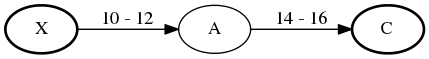
\includegraphics[width=\textwidth,height=0.5in,keepaspectratio
]{ejemplo2.png}\newline

En este caso el objetivo es llegar de X a Y con los dos vuelos disponibles. El primero  se realiza desde la ciudad X a la A . Luego, el otro parte desde A hasta C, el destino de este vuelo es la ciudad C. Como este fue el último de los disponibles, y  no llegue a Y. No hay solución.\newline \newline
\newpage
Ejemplo 3:

X Y 8\newline
vuelos:
1) Z X 1 5;  2) X A 10 22;  3) A B  24 28;  4) A B 35 41;   5) B Y 42 55;  6) X C 12 18;
7) C D 22 30;  8) D Y 34 40\newline
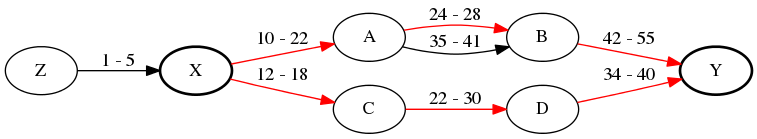
\includegraphics[width=\textwidth,height=\textheight,keepaspectratio
]{ejemplo3.png}\newline


Para llegar a X desde Y existen dos posibles itinerarios. Uno de ellos es el que contiene a los vuelos numero 2, 3, 5 y 6 ya que el tomar los vuelos en este orden me permite llegar a destino. Y entre cada uno de los vuelos se cumple que entre el horario de llegada y salida desde la misma ciudad  
haya dos horas de diferencia. Y el otro itinerario posible, es el de los vuelos 6, 7, 8. Si bien ambas son soluciones, solo el ultimo itinerario es una solución óptima al problema. Ya que, la llegada a Y se realiza 15 horas antes que en el otro itinerario y recordemos que es solución óptima el conjunto de vuelos que llega antes a destino.\newline  \newline


Ejemplo 4:

X Y 14\newline
1) X A 1 10;  2) A C 15 20;  3) C D 22 30;  4) D Y 34 40;  5) D E 32 36;  6) E Y 38 40;  7) X T 1 5;
8) T U 7 15;  9) U V 21 25 ;  10) U D 20 28;  11) V W 27 30;  12) W Z 32 35;  13)  Z S 37 41;
14) Z Y 38 40  
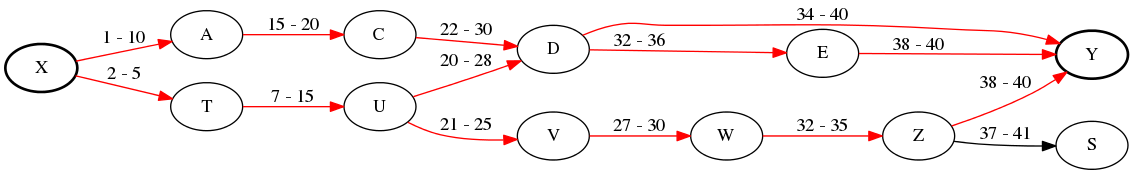
\includegraphics[width=\textwidth,height=\textheight,keepaspectratio
]{ejemplo4.png}\newline

Para este ejemplo contamos con un total de 13 vuelos. Y el objetivo es dar una solución óptima al problema de llegar desde X hasta Y. Una posible combinación de vuelos, y por lo tanto un itinerario factible, es el de los vuelos 1, 2, 3 y 4. Pero, no es el único, otro puede ser el de los vuelos 1,  2, 3, 5 y 6. También esta el que contiene a  7, 8, 9, 11, 12 y 14. y por ultimo el de los vuelos 7, 8, 10 y 4. En este caso tengo 4 itinerarios que cumple la necesidad de llegar a destino a partir de X. Edemas se puede observar que solo hay tres vuelos que llegan a destino el numero 5, 6, 14. Pero estos tres llegan a la misma hora. Entonces cualquiera de los 4 itinerarios es una solución óptima al problema.\newline \newline




\subsection{Resolución}

Como el objetivo del problema es ir de una ciudad $origen$  a una ciudad $destino$,  llegando a la misma en el menor tiempo posible y devolviendo los vuelos utilizados (se devuelven los vuelos enumerados por orden de aparición en la entrada). Teniendo una cantidad $n$, entero no negativo, de vuelos disponibles. Lo que se va a realizar en primera instancia es a cada ciudad distinta asignarle un numero entero (esto se realiza para mantener la complejidad deseada). De esta forma me van a quedar ciudades enumeras de 0 a 2*n-1, se enumeran según la posición que le toco (en el peor caso, si cada vuelos tiene ciudades distintas entonces tengo 2*n ciudades). Y se procede a tener un vector con todos los vuelos pero ahora reemplazando a las ciudad por el valor entero que le toco. Luego, se verificara que $destino$ y $origen$ existan entre los vuelos disponibles. Sino, no puedo partir o llegar desde las ciudades deseadas por lo que no habria solución. En caso contrario se ordenaran los vuelos de manera decreciente por $hora\_de\_llegada$ y se creara un vector de listas $donde$, donde las posiciones del vector representaran a cada ciudad (ciudad mapeada a un entero) y las listas en cada una, la posición donde esta ciudad es un $lugar\_de\_salida$ en $vuelos$. Tambien, un arreglo de enteros, $vuelos disponibles$, donde cada posición es una ciudad y su valor a los vuelos que hayan que partan desde dicha ciudad. Y finalmente un arreglo de bool $ya\_lo\_use$ como cada vuelo puede ser numerado apartir de la posición que se encuentra en $vuelos$ este arreglo me va a servir para informar si ya analice ese vuelo, por lo que inicialemente $ya\_lo\_use$ tendra false en todas sus posiciones. Con estas estructuras auxiliares se va a proceder a ver si existe alguna combinación entre los vuelos que me permita cumplir con el objetivo. Primero, se verifica que haya vuelos disponibles para la ciudad $origen$, si es igual a cero entonces no hay. Por ende, no hay solución. Sino, se verificara por cada vuelo que parta desde la ciudad $origen$ si tomando ese vuelo existe alguna combinación que me permita llegar a $destino$ realizada la verificación, se procede  a almacenar la posible solución en una lista, y se procede a realizar los mismo con el siguiente vuelo que parta desde $destino$ hasta el último que haya. La verificación se realiza con la función  $buscar\_llegada$. La misma va a corroborar que si la ciudad de llegada del $vuelo\_actual$ es $destino$ entonces llegue a donde quería y retorno como solución la hora de llegada y el número de vuelo, primera y segunda componente de una tupla respectivamente. Sino es así. Se verificara si existe un vuelo a partir de la ciudad de llegada de $vuelo\_actual$ que me permita llegar. Si la cantidad de vuelos disponibles para esta ciudad es cero. Entonces no llegue a destino, y ya no tengo mas vuelos para seguir, se devolverá como solución el valor -1 y una lista vacía. Si hay vuelos disponibles entonces se verificara si tomando los vuelos que salen desde esta ciudad de llegada puedo llegar a $destino$. Es decir, se llamara recursivamente a la función $buscar\_llegada$. Pero, antes de llamar a esta función se verificara que haya una diferencia de dos horas entre la hora que llego a la ciudad y el próximo vuelo que parte de esta y que no se haya trabajado con este vuelo. Si hay varios vuelos que parten de una misma ciudad y cumplen con estas condiciones, se tendrán varias soluciones dependiendo del vuelo que tome. Entonces, a cada solución se la almacenara temporalmente en una lista y se va a decrementar la cantidad de vuelos disponibles para la ciudad de la que parti en uno. Y se denota como true a la posición de $ya\_lo\_use$ para este vuelo. Cuando se terminen de recorrer todos los vuelos. Tendré una lista con posibles soluciones. Si en cada posible solución el valor de la primer componente es -1 significa que no llego a destino con esa combinación de vuelos. Si hay alguno que no lo es, a la lista que acompañe al menor valor se guarda la posición de vuelo actual y retorno esta tupla.
Finalmente al analizar todos los vuelos que salgan desde $destino$ (terminan las iteraciones del ciclo de $desde\_origen$). Verifico que haya solución,si la hay devuelvo la de menor tiempo de llegada. Ahora es cuando se utiliza la segunda componente que contiene los números de vuelos que fueron necesarios para llegar a $destino$.

\vspace{0.4cm}
\begin{algorithmic}[1]
\Procedure{Desde\_Origen}{$vector<string>$ $ciudades$, $vector<int>$ $horarios$, $string$ $origen$, $string$ $destino$}
        \State $vector<string>$ $mapeados \gets$ $\textit{devolver todas las ciudades sin repetirlas(ciudades)}$
        \State $vector<vuelo>$ $vuelos\gets$ \textit{crear vuelos asignando a cada ciudad su posición en mapeados($mapeados, ciudades, horarios$)}
        	\If{\textit{(no existe la ciudad $origen$ o $destino$ en mapeados)}}
        		\State \textit{No hay solución}
        	\Else 
        		\State $vector <list <int> > donde \gets posiciones\_de\_salida(vuelos)$
			\State bool $ya\_lo\_use[vuelos.size()]$ 
			\State \textit{asignar a cada posicion de ya\_lo\_use false(ya\_lo\_use)}       		
        		\State int vuelos\_disponibles[cantidad de ciudades distintas];
        		\For{($i$ = 0; $i$ $<$ cantidad de ciudades distintas; $i_{++}$)}
        			\State $vuelos\_disponibles[vuelos[i].lugar\_de\_salida]_{++}$
        		\EndFor	
        		\If{(vuelos\_disponibles[destino] == 0)}
        			\State \textit{No hay solución}
        		\Else	
       			\State $list$ $<tupla<int, list<int> > >$ soluciones; 
				\State $list<int> vuelos\_desde\_destino \gets donde[destino]$ 		
				\For{($iterador$ $it\gets vuelo\_desde\_destino.begin()$ to $vuelo\_desde\_destino.end()$ }
					\State $posible\_solucion\gets$ buscar\_llegada($vuelos$, $vuelos\_disponibles$, $vuelos[*it]$, $*it$,  $destino$, $donde$, $ya\_lo\_use$)
					\State soluciones.Push\_back(posible\_solucion)
				\EndFor
				\If{(no\_hay\_camino(soluciones))}
					\State \textit{no hay solucion}
				\Else
					\State return(minimo\_camino(soluciones))
				\EndIf
			\EndIf
		 \EndIf			 	
\EndProcedure
\end{algorithmic}

\vspace{0.2cm}
\begin{algorithmic}[1]

\Procedure{Buscar\_llegada}{$vector<vuelo>$ $vuelos$, $int$ $vuelos\_disponibles[]$, $vuelo$ $vuelo\_actual$, $int$ $numero\_de\_vuelo$, $int$ $destino$, $vector< list<int> >$ $donde$, $bool$ $ya\_lo\_use$}
        \State $tupla<int , list<int> >$ $itinerario$ 
        	\If{\textit{(vuelo\_actual.lugar\_de\_salida == destino)}}
        		\State $list<int>$ $camino$
        		\State return $tupla<vuelo\_actual.hora\_de\_llegada, camino.push\_back(numero\_de\_vuelo) >$
        	\Else 
        		\If{(vuelos\_disponibles[vuelo\_actual.lugar\_de\_llegada] !=0)}
       			\State $list$ $<tupla<int, list<int> > >$ soluciones;
       			\State $list<int> vuelos\_desde\_nuevo\_destino \gets donde[vuelo\_actual.lugar\_de\_llegada]$ 		 
				\For{(iterador it vuelos\_desde\_nuevo\_destino.begin() to vuelos\_desde\_nuevo\_destino.end() )}
					\If{(vuelos[*it].hora\_salida - vuelo\_actual.hora\_llegada $>=$ 2 $\&\&$ $!ya\_lo\_use[*it]$)}										
						\State $posible\_solucion\gets buscar\_llegada$
						\State soluciones.Push\_back(posible\_solucion)
						\State vuelos\_disponibles[vuelo\_actual.lugar\_de\_salida]--;
						\State ya\_lo\_use[*it]= true
					\EndIf					
				\EndFor
				\If{(no\_hay\_camino(soluciones))}
					\State itinerario.fisrt = -1
				\Else
					\State itinerario =  minimo\_camino(soluciones)
					\State itinerario.second.push\_back(numero\_de\_vuelo);
				\EndIf
			\Else
				\State itinerario.first = -1
			\EndIf
			\State return itinerario
		 \EndIf			 	
\EndProcedure
\end{algorithmic}

\subsection{Demostración de la correctitud:}

Empecemos por los casos que no tienen solución. El mismo puede suceder por varios motivos:
1)No existe la ciudad $destino$ u $origen$. Como nuestro algoritmo luego de crear el vector $vuelos$ recorre una por una todas las ciudad viendo si existen $destino$ u $origen$(linea 4 del pseudocódigo). En el caso que no existan esta sección detectaría la ausencia de algunos de los dos e inmediatamente termina con un “No hay solución”.
2) Existen las dos pero, no hay vuelos que salgan desde $origen$. El vector de listas $donde$ es el que se encarga de recorrer todos los vuelos y asignarle a cada valor que representa las ciudades de salida el número de vuelo, donde esta es un $lugar\_de\_salida$. Si $origen$ no tiene vuelos que partan desde aquí entonces la lista es vacía. Pero esto es preguntado por nuestro algoritmo y en el caso de ser vacía. Finaliza con un “No hay solución.”
3) El ultimo hecho se podría dar si no existe una forma de llegar a $destino$. Ya sea porque tomando los vuelos de salgan desde $origen$ no existe una combinación. O bien existe, pero entre alguna de los vuelos no se cumple la diferencia de horarios. Cuando existen vuelos que salen desde $destino$ o desde alguna otra ciudad que se llego por salir desde la misma. Se crea una lista provisoria para almacenar las posibles soluciones ya que en el caso  de tener muchos vuelos que salen desde una misma ciudad debo quedarme con una posible solución ($buscar\_llegada$ solo devuelve un camino). De entre las posibles  se verifica si alguna llego a $destino$. Como ya se explico si todas tienen el valor -1, No hay solución. Pero, no solo esto establece que no hay solución. Si la lista es vacía tampoco tengo solución y la función $No\_hay\_camino$ me dará como respuesta true. Entonces el ítem 3) cae en este caso. Si ninguno llega a $destino$ porque para ninguno se cumple la diferencia horaria al finalizar el ciclo que verifica si llegue a $destino$  busca en la lista la solución. Al estar vacía, porque al no cumplirse la diferencia horaria no guarde nada en la misma, se devuelve un $itinerario$ con la primer componente en -1. Y si cumple con las diferencia pero, se llega a una ciudad desde la cual ya no hay vuelos de salida y dicha ciudad no es $destino$. Entonces, los vuelos disponibles para dicha ciudad deben ser igual a cero. Cuando esto sucede también se devuelve el valor -1. Denotando que no hay solución. Lo primordial recae en que el valor de la primer componente de la tupla va a ser distinto de -1 solo si se llego a destino. En cualquier  otro caso tiene el valor -1. Y si sucede esto se interpreta que tomando esos vuelos No hay solución.
Estos son todos los casos en los cuales el problema no tiene solución y el algoritmo es capaz de detectar cada uno de ellos.
Caso: Hay solución:
No solo nos importa que el algoritmo devuelva una solución si la hay, sino que  esta sea la óptima.
Primero empezaremos por destacar que siempre sea posible todos los vuelos que se pueden llegar a partir de $destino$. Para cumplir con esto esta el vector de lista $donde$. El mismo representa el numero de los vuelos que salen desde cada ciudad (siendo la ciudad la posición del vector $donde$). Por lo que la suma de las longitudes de todas las listas es igual a n ya que representa todos los vuelos que salen desde cada una. Y nuestro algoritmo para encontrar el camino que me conduce hasta $destino$ posee un ciclo que se  ejecuta para cada uno de estos valores. Así cada vez que lleguemos a una ciudad exploraremos todos los vuelos que salen desde esta. Y en el caso de que se cumpla la diferencia de horarios. Seguiremos explorando ahora con estos nuevos vuelos. El tener este vector además me asegura de analizar todos los vuelos que salen desde $destino$. Esto se ejecuta en la función $desde\_origen$, en la linea 19 del pseudocódigo dado. Se observa que se ejecuta para cada uno de los vuelos que parten desde $destino$. Entonces hasta el momento tenemos que siempre se van a analizar todos los vuelos que salen desde $destino$ y para cada una de las ciudades a las que se llega, se recorren (de ser posibles) todos los vuelos que parten desde estas. Así hasta que la ciudad de llegada del vuelo que se esta analizando $vuelo actual$ sea $destino$( que sabemos que aunque sea un vuelo llega por que estamos en ese caso). Entonces al analizar todos los vuelos sabemos que vamos a llegar a $destino$. Ahora queremos corroborar que esta información no se pierde y que por cada iteración realizada en $desde\_origen$ si se llega a $destino$ tomando ese vuelo me devuelva el menor de los caminos con esa combinación.
Vamos a suponer dos casos:
1) Al tomar un vuelo que parte desde $origen$ es posible llegar a $destino$ y para cada ciudad a la cual se llega solo existe un solo vuelo de salida. Es decir, sea la ciudad X, la ciudad de llegada del vuelo que parte desde $destino$, luego solo hay un vuelo que sale desde X, llegando a la ciudad Y, y para esta ocurre lo mismo. Así hasta llegar a $destino$. Cuando llegamos se crea una lista que va a ir almacenando a cada uno de los vuelos que utilice para llegar hasta aquí. Y se devolverá una tupla con esta lista y el horario de llegada. Ahora la función que llamo a esta instancia evaluara el valor de la tupla. Como el valor es distinto de -1, ya que se guardo el horario y este es un entero no negativo, el algoritmo detecta que llegue  a $destino$ por lo que procede a guardar en la lista el numero de este vuelo. Lo mismo va a suceder hasta volver al vuelo con $origen$ como partida. Luego de esto se almacena  esta tupla con el horario de llegada y la lista de vuelos usados en la lista ,$soluciones$, provisoria para su posterior análisis.
Si solo se tiene este vuelo que parte desde $origen$ entonces, $no\_hay\_solucion$ dará false porque hay un valor distinto de -1. y $minimo_camino$ devolverá esta tupla ya que es la única. Y por ende la única solución óptima. Si hay mas vuelos y cada uno con la misma característica (de cada ciudad solo hay un vuelo de salida) entonces sucederá lo mismo encontrara el camino guardara el horario y   los vuelos utilizados. Y $minimo\_camino$ va a devolver aquel cuya componente sea la menor y distinta a -1. Como solo se cambia el valor cuando llego a destino. Si como solución final retorno a aquella tupla cuyo valor sea el mínimo y distinto a -1 estoy devolviendo el vuelo que antes llega a $destino$ la solución óptima. Puede ocurrir que uno de los vuelos utilice un camino que ya se uso pero, si esto sucede entonces ya tengo la solución almacenada por lo que no afecta que ahora establezca que no hay camino con ese vuelo.
Por ultimo esta el caso en el de que de una ciudad salgan varios vuelos. Pero, cuando esto suceda se puede pensar como que esta es mi nueva ciudad  $destino$. Es decir se piensa el problema en general pero para instancias más chicas. Teniendo un nuevo $destino$ se evaluaran todos los vuelos que parten desde esta y nos quedaremos al igual que en el caso para el problema original, con la tupla cuya primer componente es la mínima. Finalizada la instancia mas chica, la otra que la contiene ya tendrá la solución óptima para esa combinación de vuelos, lo mismo sucederá para la que contiene a esta. Así hasta llegar nuevamente a la instancia general. Que es la que tiene como partida a $destino$ nuevamente se almacenara la solución. Y se devolverá la menor. De esta manera el algoritmo siempre encuentra los caminos que llegan a $destino$ y devuelve el que llega antes.

\subsection{Análisis de complejidad temporal:}

Para calcular la complejidad total vamos a analizar por partes nuestro algoritmo.\newline
1) La funcion principal $desde\_origen$ recibe dos vectores. Uno de ellos de string que representa a las ciudades, $ciudades$ y otro las hora de salida y llegada $horarios$. Como ya se menciono, cada ciudad distinta sera mapeada a un valor entero. Para esto se procede a crear una lista con las ciudades, de manera que en esta no haya ciudades repetidas. Entonces, tendre a lo sumo 2*n ciudades y según la posición que ocupe cada ciudad sera el numero que se le asignara. El costo de esto, fue crear la lista con las ciudades sin repetidos,  O(2*n) tamaño de la lista. Más verificar no introducir una ciudad repetida para esto, si estoy recorriendo la posición i-esima de $ciudades$, 1$<=$ $i$ $<$ n,  me fijo si a esta i-esima ciudad no la analice antes, es decir desde la posición 0 a i-1. \newline
$\sum_{i=0}^{2*n}{i}= O(n^{2})$\newline
2) Teniendo un valor entero que representa a cada ciudad se construye el vector $vuelos$ del tipo  vuelo. A medida que se recorre el vector de ciudades y de horarios, avanzo de a par, la primer posición de este par en $ciudades$ es el $lugar\_de\_salida$, y el segunda el $lugar\_de\_llegada$ mientras que en el otro vector representa $horario\_de\_salida$, $horario\_de\_llegada$ respectivamente todo para un mismo vuelo. Pero antes de construir el vuelo las ciudades en cuestión  deben ser con su asignacion al valor entero. Para esto se debe buscar en mapeados la posición que ocupa la ciudad. Complejidad:
O(2*n) + O(2*n) que buscar por cada ciudad, de origen y de llegada, el valor entero que tiene asignado, siendo el tamaño de mapeados a lo sumo 2*n. Y esto se realiza para todas las ciudades 0(2*n*(O(2*n) + O(2*n))) = O($n^{2}$).\newline
3) Verificar si existen las ciudades $destino$ y $origen$. Complejidad: O(2*n).O(1) Recorrer mapeado por el costo de verificar si las ciudades existen, comparar string.\newline
4) Crear el vector de listas de int $donde$, mediante el uso de la funcion auxiliar $posiciones\_en\_vuelo$. Se recorre el vector $vuelos$ y por cada vuelo a donde[$lugar\_de\_salida]$, se le guarda la posición de este vuelo en $vuelos$, es decir si estamos en la i-esima iteracion del vector vuelos, 0$<=$ $i$ $<$ n. se guarda el valor i (recordemos que ahora los vuelos son del tipo entero de 0 a 2*n-1, en el peor caso, por lo que cada cada valor se asocia a una posición). Complejidad : O(n).O(1) (recorrer el vector vuelos por lo que cuesta guardar las posiciones que son push\_back en cada lista.)\newline
5) Crear el arreglo $ya\_lo\_use$ que tiene el mismo tamaño que la cantidad de vuelos disponibles. Y a cada posición hay que asignarle el valor false: O(n) en total\newline
6) Construir el vector $vuelos\_disponibles$, el mismo es de tamaño de $mapeados$ ya que por cada  ciudad quiero indicar la cantidad de vuelos que salgan desde esta ciudad. Por lo que la resolución es similar al item 5). se recorre $vuelos$ pero ahora en vez de guardarme la posición incremento en uno el valor de la posición (inicialmente todas estan en cero) que represente el lugar\_de\_salida. Complejidad O(n) (recorrer vuelos e incrementar el valor O(1)). \newline
7) verificar que haya vuelos disponibles desde destino, O(1) me fijo si el tamaño de la lista para $donde[destino]$ es == 0. Se utiliza la instrucción $empty()$ provista por la stl.\newline
8) Verificar si hay alguna combinacion de vuelos que me permita llegar a destino. Como se hace uso de una funcion recursiva, $buscar\_llegada$. Primero vamos a analizar la complejidad de lo que se realiza en cada llamada.\newline
8.a) $buscar\_llegada$ devuelve una $tupla<int, list<int>>$ $itinerario$, la primer componente tendra el horario de llegada si es que hay un camino hacia $destino$ y la segunda el numero de los vuelos que me permiten llegar. En caso contrario solo tendrá el valor -1. Si llegué a $destino$, a la primer componente se le asigna el horario de llegada del vuelo actual O(1), se crea la lista que va a tener a los números de vuelo y se pushea $numero\_de\_vuelo$ O(1).\newline
8.b) Si no se llego a $destino$, y la cantidad de vuelos disponibles para la ciudad de llegada de $vuelo\_actual$ es distinta de cero. Entonces, significa que existen vuelos que parten desde esta ciudad. Se evaluaran los mismos haciendo tantas llamadas a la funcion $buscar\_llegada$ como vuelos hayan (los que salgan desde esta ciudad). Los mismos se conocen por $donde$, solo basta buscar a este vuelo en la estructura. Usando $donde[vuelo\_actual.lugar\_de\_salida]$ ya los tengo (este es el principal de uso de tener mapeadas las ciudades a un valor entero, puedo obtener esta información en O(1)). Al ya tener los vuelos que debo analizar se procede a realizar un for que verifique con cada uno de estos si puedo llegar a $destino$. Luego de cada llamada se guardara la posible solución en una lista provisoria (luego se realizara un análisis del costo de guardar estas posibles soluciones). La verificación con los mismos se realizara si cumplen dos condiciones. La primera es la diferencia de horario (requisito necesario por el problema) 0(1). La segunda es que, ya no se haya analizado este vuelo porque si se analizo entonces estaría repiento la busqueda que ya analice y es necesario para nuestra complejidad que los vuelos solo se analicen una sola vez O(1) basta ver si $ya\_lo\_use[numero\_de\_vuelo]$ es igual a false. Cuando los vuelos se analizan se disminuye la cantidad de vuelos disponibles de la ciudad de llegada del $vuelo actual$ O(1). Y a $ya\_lo\_use[numero\_de\_vuelo]$ se le asigno true para que si otra combinacion de vuelos hace uso de este, ya se sabe que se analizo y no tener que calcular nuevamente lo mismo. Para poder cumplir con que los vuelos se analicen una sola vez es que se tiene el vector $ya\_lo\_use$ y $vuelos\_disponibles$. si un vuelo $t$ cumple con la condición sobre la diferencia horaria voy a poder analizar todos los vuelos que salgan de esta ciudad y la cantidad de vuelos disponibles para la posición $t.lugar\_de\_llegada$ va a ser igual a cero. Por lo que si hay otros vuelos que luego utilicen a $t$ como vuelo escala, al verificar si hay vuelos disponibles tendran que no, (que es igual a cero). De esta forma me aseguro de no realizar análisis repetido. Ahora bien, puede que el vuelo que este analizando no cumpla con la diferencia horaria para todos los vuelos pero si para algunos, es por eso que ádemas se cuenta con $ya\_lo\_use$. Para los vuelos que se puedan verificar entonces se los verificará y se tendrá marcado que ya los revisaron así los posterior vuelos no necesitan volver a revisar estos sino, aquellos que en su momento no se pudieron hacer por no cumplir la diferencia horaria. Luego, de tener para la instancia de vuelo $t$ todas las posibles soluciones se procede a verificar si hay solución y si la hay, cual es. Para esto primero se verifica que todas las posibles soluciones no tengan el valor -1 en su primer componente. Si es asi entonces no hay solucion y se devuelve la tupla creada al principio $itinerario$ con el valor -1 en su primer componente. En caso de que la haya se recorre todas las soluciones y se devuelve el menor valor distinto de -1. Ambas funciones son lineales en la cantidad de posibles soluciones, y esta cantidad es igual a los vuelos que parten desde $t$.lugar\_de\_llegada. La cantidad de posibles vuelos que partan desde una misma ciudad, para todos los n vuelos, es igual a n, ya que son todos los vuelos que existen. Como se analizan por cada iteración del ciclo de $desde\_origen$ a lo sumo una vez cada vuelo y luego si se necesita de un vuelo que ya fue analizado con ver la cantidad de vuelos disponibles, o ya\_fue\_usado basta, en el peor de los casos averiguar si ya fue usado se lo voy a preguntar a todos los vuelos O(n), pero esto ocurre por cada iteración de $desde\_origen$. En el peor de los casos si son c los vuelos desde $destino$ entonces seria c.O(n) acotando c por n tenemos O($n^{2}$). \newline
8.c)Finalmente analizamos la complejidad de guadar las posibles soluciones. Al guardar esto, si bien se utiliza la funcion push\_back() en la lista provisoria. Se esta guardando una tupla que posee una lista con los vuelos usados para llegar a $destino$. Si es que hay camino sino, solo una tupla con una lista vacia y esto se hace en O(1). En el otro caso es lineal a la cantidad de elementos en la lista. Entonces como cada vuelo se analiza a lo sumo sola vez, en todas las iteraciones estaremos realizando copias con valores distintos. No podria haber como solución un vuelo que este tambien como solucion para otro camino ya que cuando se lo analizó por primera vez se puso que ya fue usado este vuelo en $ya\_lo\_use$ y en este caso nuestro algoritmo plantea que no hay solución porque ya se analizo el mismo y ya se conoce su resultado . Entonces, si al finalizar todas las iteraciones de $desde\_origen$ se tienen k posibles soluciones, (k igual a los vuelos disponibles desde $destino$). Significa que tengo k listas que fueron copiadas tantas veces como vuelos se necesitaron para llegar a $destino$. Suponemos el peor caso, que todos los vuelos llegan a destino entonces la suma de las longitudes de esas listas es n, (por lo argumentado anteriormente no se utilizan vuelos que hayan en otras soluciones). Entonces, si pensamos ahora todo como una sola lista y suponemos que fue copiada tantas veces como la máxima vez que fue copiada algunas de las k listas. Y sabemos que las listas se copiaron a lo sumo n veces porque se van insertando de a uno cada nuevo $numero\_de\_vuelo$ 
tenemos que la complejidad de todas las copias son:\newline
$\sum_{i=0}^{2*n}{i}= O(n^{2})$\newline
\textit{cada vez que voy a agregar un nuevo número de vuelo copio todos los anteriores}\newline
8.d)Finalizadas todas las llamadas a la función recursiva, se procede a verificar cual de las k soluciones es la correcta, utilizando nuevamente si existe solución y cual es. Ambas lineales en la cantidad de posibles soluciones O(k), acotando k por n tenemos O(n)\newline
juntando las complejidades de los casos 1-8 tenemos que la complejidad total es:     

$O(n^{2})$ + $O(n^{2})$ + $O(2*n)$ + $O(2*n)$ + $O(n)$ + $O(2*n)$ + $O(1)$ + $O(1)$ +$O(n^{2})$ + $O(n^{2})$ + $O(n)$  = $O(4*n^{2})$ + $O(2*n)$ + $O(2)$ + $(3*2*n)$ = $O(n^{2})$ =  $O(n^{2})$
\subsection{Recursos utilizados:}
\begin{itemize}
\item Crear una lista vacía tiene complejidad constante \newline (http://en.cppreference.com/w/cpp/container/list/list caso 1)
\item AgregarAtras a una lista tiene complejidad constante 
\newline (http://en.cppreference.com/w/cpp/container/list/push\_back)
\item Asignar, incrementar y comparar enteros tiene complejidad constante
\item Preguntar si una lista es vacía tiene complejidad constante \newline (http://en.cppreference.com/w/cpp/container/list/empty)
\item Pedir el iterador al inicio de una lista y al final tienen complejidad constante \newline (http://en.cppreference.com/w/cpp/container/list/begin, http://en.cppreference.com/w/cpp/container/list/end). Avanzarlos y crearlos también ya que son punteros a nodos de la lista. 
\item Asignar a una lista $l1$, otra lista $l2$ tiene complejidad lineal a $|l2|$ \newline (http://en.cppreference.com/w/cpp/container/list/operator\%3D)
\end{itemize}

\subsection{Experimentación:}


En la sección análisis de la complejidad se demostró que la complejidad del problema es $O(n^{2})$. Para verificar esto en la practica, se procedió a calcular la perfomance de nuestro algoritmo, en milisegundos, a partir del tiempo que tarda en resolver distintas instancias del problema. El mismo se ejecutó para una cantidad que va desde un vuelo a quinientos y se repitió este procedimiento 5 veces. Se realizaron un total de 3 gráficos. El primero \textit{gráfico 1} representa el tiempo que tardo en ejecutarse para las instancias mencionadas representando en el  mismo el tiempo máximo, mínimo y promedio. En el \textit{gráfico 2}, a los tiempos calculados en el primero se los dividió por la cantidad de vuelos según la instancia que se representaba también con tiempo mínimo, máximo y promedio. Finalmente el \textit{gráfico 3} refleja el tiempo que tardo dividido  $cantidad$ $de$ $vuelos^{2}$, al igual que en los anteriores con tiempo máximo, mínimo y promedio.   

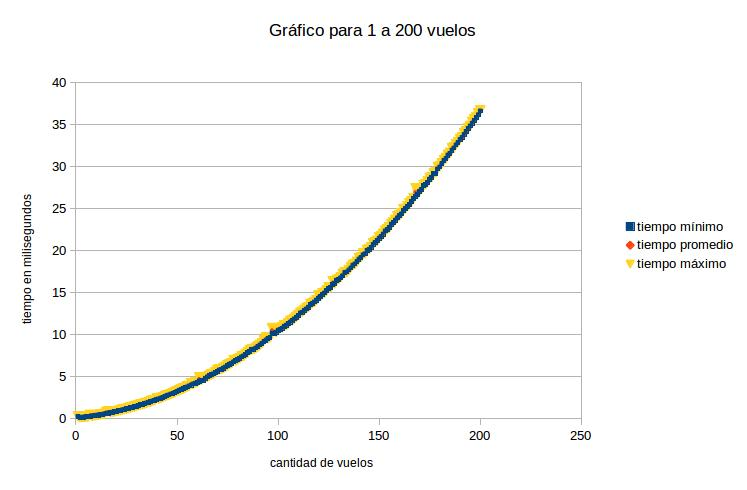
\includegraphics[height=3.5in,height=3.5in,keepaspectratio
]{normal.jpg}\newline
gráfico 1: Se puede observar como el tiempo máximo sobresale muy levemente sobre el mínimo superponiéndose al promedio.Se puede observar que los mismos generan una curva.Para confirmar que tiene un comportamiento cuadrático se divide por la cantidad de vuelos. Por lo que el nuevo gráfico deberia representar una recta. \newline

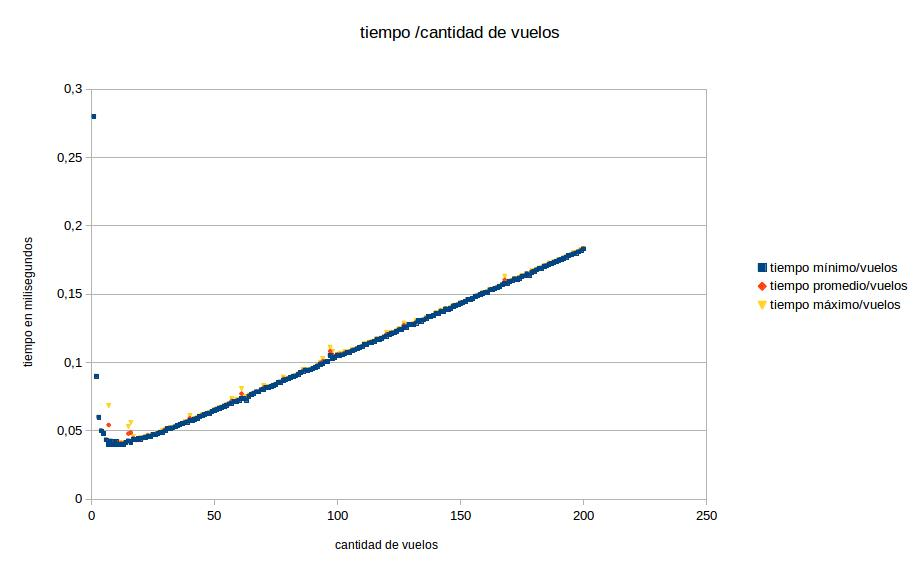
\includegraphics[width=\textwidth,height=\textheight,keepaspectratio
]{divididon.jpg}\newline
gráfico 2: Al dividir los tiempos por la cantidad de vuelos se oberva que para los tiempos observables que son el mínimo y el máximo, mientras que el promedio se encuentra tapados por estos. Los mismos generan una recta. Si bien, al principio se observan algunos picos a medida que la cantidad de vuelos aumenta estos valores no difieren mucho entre si generando una recta casi sin valores que sobresalgan de la misma.\newline
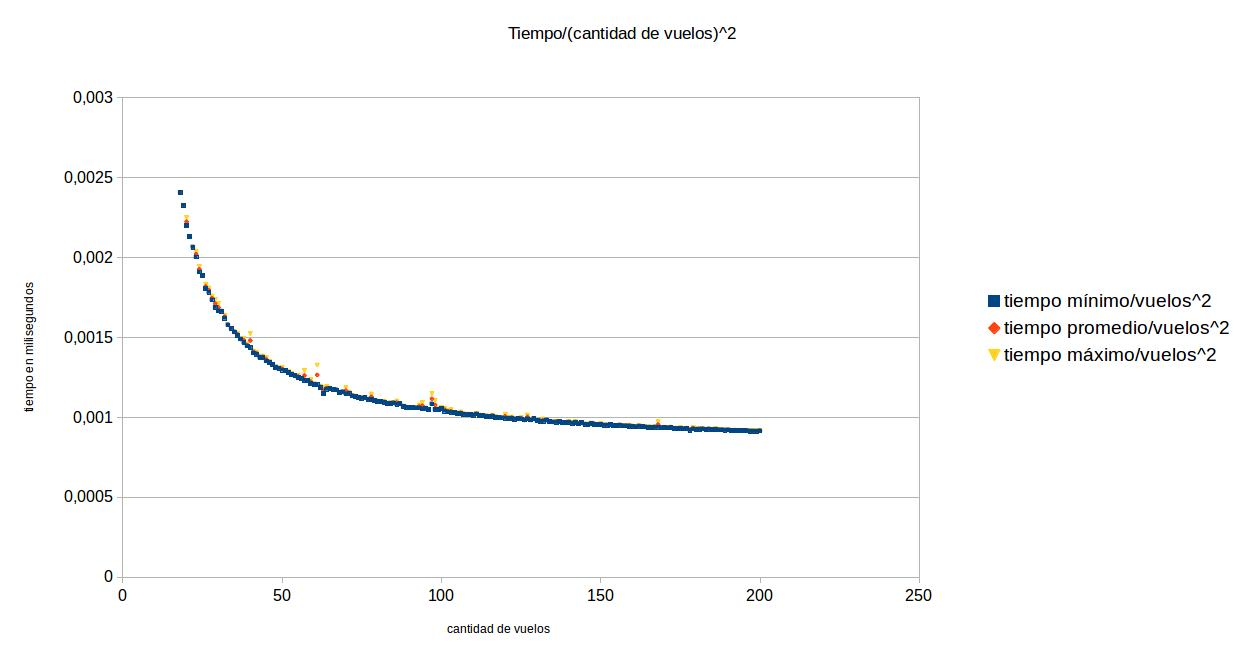
\includegraphics[width=\textwidth,height=\textheight,keepaspectratio
]{porcuadrado.jpg}\newline
gráfico 3: Finalmente para corroborar que la complejidad es $n^{2}$, siendo n la cantidad de vuelos, a los tiempos se lo dividido por $n^{2}$, de esta forma el gráfico debería quedar una constante. En el mismo se puede observar que para los primero valores se asemeja a una curva ya que los valores empiezan a decrecer rápidamente. Pero, a medida que la cantidad de vuelos aumentan los valores empiezan a disminuir lentamente y empezando a converger a un solo valor a medida que estos crecen. Es decir, a una constante que era el comportamiento que deseábamos.

\end{document}